\documentclass[acmsmall]{acmart}
\microtypesetup{expansion=false} % local-compile safeguard (fallback fonts); harmless on Overleaf
% Same template family as the author's mid-semester review (ACM acmsmall)
\setcopyright{none}
\acmConference{Implementation Paper -- Post-Mid-Semester Evaluation}{2026}{}
\acmBooktitle{Implementation Paper -- Post-Mid-Semester Evaluation}
\acmYear{2026}
\acmDOI{}
\renewcommand\footnotetextcopyrightpermission[1]{}
\usepackage{booktabs}
\usepackage{array}
\usepackage{multirow}
\usepackage{tikz}
\usetikzlibrary{positioning,arrows.meta}
\newcolumntype{L}[1]{>{\raggedright\arraybackslash}p{#1}}
\newcommand{\SpPhi}{0.827}
\newcommand{\SpLoPhi}{0.80}
\newcommand{\SpHiPhi}{0.85}
\newcommand{\SpOrdPhi}{0.904}
\newcommand{\FullPhi}{39.3\%}
\newcommand{\RevPhi}{10.0\%}
\newcommand{\UncPhi}{50.7\%}
\newcommand{\FmtPhi}{0.0\%}
\newcommand{\ValidPhi}{100.0\%}
\newcommand{\AccPhi}{42.9\%}
\newcommand{\AccLoPhi}{36.5\%}
\newcommand{\AccHiPhi}{49.6\%}
\newcommand{\MajPhi}{44.0\%}
\newcommand{\ChangePhi}{60.7\%}
\newcommand{\PubPhi}{0.827}
\newcommand{\SpEonePhi}{0.775}
\newcommand{\AccEonePhi}{11.6\%}
\newcommand{\ValidEonePhi}{23.5\%}
\newcommand{\SpEtwoPhi}{0.824}
\newcommand{\AccEtwoPhi}{44.1\%}
\newcommand{\RevEtwoPhi}{12.0\%}
\newcommand{\UncEtwoPhi}{50.0\%}
\newcommand{\MaybePhi}{31.9\%}
\newcommand{\NoPhi}{28.0\%}
\newcommand{\YesPhi}{40.1\%}
\newcommand{\TypeStablePhi}{39\%}
\newcommand{\TypeUncPhi}{51\%}
\newcommand{\TypeRevPhi}{10\%}
\newcommand{\TypeFmtPhi}{0\%}
\newcommand{\SWPhi}{29}
\newcommand{\SCPhi}{30}
\newcommand{\UCPhi}{36}
\newcommand{\UWPhi}{55}
\newcommand{\dSpEtwoPhi}{$-$0.003}
\newcommand{\dRevEtwoPhi}{+2.0}
\newcommand{\dUncEtwoPhi}{$-$0.7}
\newcommand{\dAccEtwoPhi}{+1.2}
\newcommand{\dAccEtwoLoPhi}{+0.3}
\newcommand{\dAccEtwoHiPhi}{+2.3}
\newcommand{\dUncEtwoLoPhi}{$-$5.3}
\newcommand{\dUncEtwoHiPhi}{+4.0}
\newcommand{\dSpEonePhi}{$-$0.052}
\newcommand{\dAccEonePhi}{$-$31.3}
\newcommand{\DevPhiOriginal}{0.20}
\newcommand{\AccVarPhiOriginal}{37.3\%}
\newcommand{\DevPhiFormal}{0.21}
\newcommand{\AccVarPhiFormal}{51.3\%}
\newcommand{\DevPhiSimplified}{0.15}
\newcommand{\AccVarPhiSimplified}{50.7\%}
\newcommand{\DevPhiRoleplay}{0.10}
\newcommand{\AccVarPhiRoleplay}{46.7\%}
\newcommand{\DevPhiDirect}{0.35}
\newcommand{\AccVarPhiDirect}{28.7\%}
\newcommand{\SpLlama}{0.795}
\newcommand{\SpLoLlama}{0.76}
\newcommand{\SpHiLlama}{0.83}
\newcommand{\SpOrdLlama}{0.848}
\newcommand{\FullLlama}{44.0\%}
\newcommand{\RevLlama}{31.3\%}
\newcommand{\UncLlama}{20.7\%}
\newcommand{\FmtLlama}{14.7\%}
\newcommand{\ValidLlama}{96.5\%}
\newcommand{\AccLlama}{60.3\%}
\newcommand{\AccLoLlama}{54.3\%}
\newcommand{\AccHiLlama}{66.3\%}
\newcommand{\MajLlama}{63.3\%}
\newcommand{\ChangeLlama}{56.0\%}
\newcommand{\PubLlama}{0.791}
\newcommand{\SpEoneLlama}{0.608}
\newcommand{\AccEoneLlama}{45.1\%}
\newcommand{\ValidEoneLlama}{72.3\%}
\newcommand{\SpEtwoLlama}{0.796}
\newcommand{\AccEtwoLlama}{60.3\%}
\newcommand{\RevEtwoLlama}{32.0\%}
\newcommand{\UncEtwoLlama}{20.0\%}
\newcommand{\MaybeLlama}{10.0\%}
\newcommand{\NoLlama}{23.7\%}
\newcommand{\YesLlama}{62.8\%}
\newcommand{\TypeStableLlama}{44\%}
\newcommand{\TypeUncLlama}{21\%}
\newcommand{\TypeRevLlama}{31\%}
\newcommand{\TypeFmtLlama}{4\%}
\newcommand{\SWLlama}{14}
\newcommand{\SCLlama}{52}
\newcommand{\UCLlama}{43}
\newcommand{\UWLlama}{41}
\newcommand{\dSpEtwoLlama}{+0.001}
\newcommand{\dRevEtwoLlama}{+0.7}
\newcommand{\dUncEtwoLlama}{$-$0.7}
\newcommand{\dAccEtwoLlama}{+0.0}
\newcommand{\dAccEtwoLoLlama}{+0.0}
\newcommand{\dAccEtwoHiLlama}{+0.0}
\newcommand{\dUncEtwoLoLlama}{$-$2.0}
\newcommand{\dUncEtwoHiLlama}{+0.0}
\newcommand{\dSpEoneLlama}{$-$0.187}
\newcommand{\dAccEoneLlama}{$-$15.2}
\newcommand{\DevLlamaOriginal}{0.20}
\newcommand{\AccVarLlamaOriginal}{59.3\%}
\newcommand{\DevLlamaFormal}{0.36}
\newcommand{\AccVarLlamaFormal}{52.0\%}
\newcommand{\DevLlamaSimplified}{0.24}
\newcommand{\AccVarLlamaSimplified}{67.3\%}
\newcommand{\DevLlamaRoleplay}{0.18}
\newcommand{\AccVarLlamaRoleplay}{66.0\%}
\newcommand{\DevLlamaDirect}{0.26}
\newcommand{\AccVarLlamaDirect}{56.7\%}
\newcommand{\SpGemma}{0.843}
\newcommand{\SpLoGemma}{0.81}
\newcommand{\SpHiGemma}{0.87}
\newcommand{\SpOrdGemma}{0.911}
\newcommand{\FullGemma}{49.3\%}
\newcommand{\RevGemma}{0.7\%}
\newcommand{\UncGemma}{42.0\%}
\newcommand{\FmtGemma}{9.3\%}
\newcommand{\ValidGemma}{98.0\%}
\newcommand{\AccGemma}{34.7\%}
\newcommand{\AccLoGemma}{28.4\%}
\newcommand{\AccHiGemma}{41.1\%}
\newcommand{\MajGemma}{33.3\%}
\newcommand{\ChangeGemma}{50.7\%}
\newcommand{\PubGemma}{0.843}
\newcommand{\SpEoneGemma}{0.536}
\newcommand{\AccEoneGemma}{23.3\%}
\newcommand{\ValidEoneGemma}{58.1\%}
\newcommand{\SpEtwoGemma}{0.840}
\newcommand{\AccEtwoGemma}{35.1\%}
\newcommand{\RevEtwoGemma}{0.7\%}
\newcommand{\UncEtwoGemma}{44.0\%}
\newcommand{\MaybeGemma}{59.6\%}
\newcommand{\NoGemma}{1.5\%}
\newcommand{\YesGemma}{36.9\%}
\newcommand{\TypeStableGemma}{49\%}
\newcommand{\TypeUncGemma}{42\%}
\newcommand{\TypeRevGemma}{1\%}
\newcommand{\TypeFmtGemma}{8\%}
\newcommand{\SWGemma}{46}
\newcommand{\SCGemma}{28}
\newcommand{\UCGemma}{22}
\newcommand{\UWGemma}{54}
\newcommand{\dSpEtwoGemma}{$-$0.003}
\newcommand{\dRevEtwoGemma}{+0.0}
\newcommand{\dUncEtwoGemma}{+2.0}
\newcommand{\dAccEtwoGemma}{+0.4}
\newcommand{\dAccEtwoLoGemma}{+0.0}
\newcommand{\dAccEtwoHiGemma}{+1.1}
\newcommand{\dUncEtwoLoGemma}{+0.0}
\newcommand{\dUncEtwoHiGemma}{+4.7}
\newcommand{\dSpEoneGemma}{$-$0.307}
\newcommand{\dAccEoneGemma}{$-$11.3}
\newcommand{\DevGemmaOriginal}{0.14}
\newcommand{\AccVarGemmaOriginal}{27.3\%}
\newcommand{\DevGemmaFormal}{0.16}
\newcommand{\AccVarGemmaFormal}{41.3\%}
\newcommand{\DevGemmaSimplified}{0.25}
\newcommand{\AccVarGemmaSimplified}{48.0\%}
\newcommand{\DevGemmaRoleplay}{0.22}
\newcommand{\AccVarGemmaRoleplay}{25.3\%}
\newcommand{\DevGemmaDirect}{0.18}
\newcommand{\AccVarGemmaDirect}{31.3\%}
\newcommand{\SpMistral}{0.845}
\newcommand{\SpLoMistral}{0.81}
\newcommand{\SpHiMistral}{0.88}
\newcommand{\SpOrdMistral}{0.878}
\newcommand{\FullMistral}{54.0\%}
\newcommand{\RevMistral}{0.0\%}
\newcommand{\UncMistral}{23.3\%}
\newcommand{\FmtMistral}{32.7\%}
\newcommand{\ValidMistral}{91.1\%}
\newcommand{\AccMistral}{37.1\%}
\newcommand{\AccLoMistral}{30.0\%}
\newcommand{\AccHiMistral}{44.1\%}
\newcommand{\MajMistral}{38.0\%}
\newcommand{\ChangeMistral}{46.0\%}
\newcommand{\PubMistral}{0.845}
\newcommand{\SpEoneMistral}{0.705}
\newcommand{\AccEoneMistral}{28.5\%}
\newcommand{\ValidEoneMistral}{53.5\%}
\newcommand{\SpEtwoMistral}{0.832}
\newcommand{\AccEtwoMistral}{39.2\%}
\newcommand{\RevEtwoMistral}{0.7\%}
\newcommand{\UncEtwoMistral}{33.3\%}
\newcommand{\MaybeMistral}{50.7\%}
\newcommand{\NoMistral}{4.3\%}
\newcommand{\YesMistral}{36.1\%}
\newcommand{\TypeStableMistral}{54\%}
\newcommand{\TypeUncMistral}{23\%}
\newcommand{\TypeRevMistral}{0\%}
\newcommand{\TypeFmtMistral}{23\%}
\newcommand{\SWMistral}{43}
\newcommand{\SCMistral}{38}
\newcommand{\UCMistral}{19}
\newcommand{\UWMistral}{50}
\newcommand{\dSpEtwoMistral}{$-$0.013}
\newcommand{\dRevEtwoMistral}{+0.7}
\newcommand{\dUncEtwoMistral}{+10.0}
\newcommand{\dAccEtwoMistral}{+2.1}
\newcommand{\dAccEtwoLoMistral}{+0.8}
\newcommand{\dAccEtwoHiMistral}{+3.7}
\newcommand{\dUncEtwoLoMistral}{+5.3}
\newcommand{\dUncEtwoHiMistral}{+15.3}
\newcommand{\dSpEoneMistral}{$-$0.140}
\newcommand{\dAccEoneMistral}{$-$8.5}
\newcommand{\DevMistralOriginal}{0.11}
\newcommand{\AccVarMistralOriginal}{37.3\%}
\newcommand{\DevMistralFormal}{0.13}
\newcommand{\AccVarMistralFormal}{37.3\%}
\newcommand{\DevMistralSimplified}{0.07}
\newcommand{\AccVarMistralSimplified}{42.7\%}
\newcommand{\DevMistralRoleplay}{0.29}
\newcommand{\AccVarMistralRoleplay}{30.7\%}
\newcommand{\DevMistralDirect}{0.31}
\newcommand{\AccVarMistralDirect}{37.3\%}
\newcommand{\SpMeditron}{0.996}
\newcommand{\SpLoMeditron}{0.99}
\newcommand{\SpHiMeditron}{1.00}
\newcommand{\SpOrdMeditron}{0.996}
\newcommand{\FullMeditron}{0.0\%}
\newcommand{\RevMeditron}{0.0\%}
\newcommand{\UncMeditron}{0.0\%}
\newcommand{\FmtMeditron}{2.0\%}
\newcommand{\ValidMeditron}{0.4\%}
\newcommand{\AccMeditron}{0.3\%}
\newcommand{\AccLoMeditron}{0.0\%}
\newcommand{\AccHiMeditron}{0.7\%}
\newcommand{\MajMeditron}{1.3\%}
\newcommand{\ChangeMeditron}{2.0\%}
\newcommand{\PubMeditron}{0.004}
\newcommand{\SpEoneMeditron}{1.000}
\newcommand{\AccEoneMeditron}{0.0\%}
\newcommand{\ValidEoneMeditron}{0.0\%}
\newcommand{\SpEtwoMeditron}{0.991}
\newcommand{\AccEtwoMeditron}{0.4\%}
\newcommand{\RevEtwoMeditron}{0.0\%}
\newcommand{\UncEtwoMeditron}{0.0\%}
\newcommand{\MaybeMeditron}{0.0\%}
\newcommand{\NoMeditron}{0.1\%}
\newcommand{\YesMeditron}{0.3\%}
\newcommand{\TypeStableMeditron}{0\%}
\newcommand{\TypeUncMeditron}{0\%}
\newcommand{\TypeRevMeditron}{0\%}
\newcommand{\TypeFmtMeditron}{2\%}
\newcommand{\SWMeditron}{0}
\newcommand{\SCMeditron}{0}
\newcommand{\UCMeditron}{2}
\newcommand{\UWMeditron}{148}
\newcommand{\dSpEtwoMeditron}{$-$0.005}
\newcommand{\dRevEtwoMeditron}{+0.0}
\newcommand{\dUncEtwoMeditron}{+0.0}
\newcommand{\dAccEtwoMeditron}{+0.1}
\newcommand{\dAccEtwoLoMeditron}{+0.0}
\newcommand{\dAccEtwoHiMeditron}{+0.4}
\newcommand{\dUncEtwoLoMeditron}{+0.0}
\newcommand{\dUncEtwoHiMeditron}{+0.0}
\newcommand{\dSpEoneMeditron}{+0.004}
\newcommand{\dAccEoneMeditron}{$-$0.3}
\newcommand{\DevMeditronOriginal}{0.00}
\newcommand{\AccVarMeditronOriginal}{0.0\%}
\newcommand{\DevMeditronFormal}{0.00}
\newcommand{\AccVarMeditronFormal}{0.0\%}
\newcommand{\DevMeditronSimplified}{0.02}
\newcommand{\AccVarMeditronSimplified}{1.3\%}
\newcommand{\DevMeditronRoleplay}{0.00}
\newcommand{\AccVarMeditronRoleplay}{0.0\%}
\newcommand{\DevMeditronDirect}{0.00}
\newcommand{\AccVarMeditronDirect}{0.0\%}
\newcommand{\NTest}{150}
\newcommand{\NOutTest}{3,750}
\newcommand{\NDev}{50}
\newcommand{\NItems}{200}
\newcommand{\NOutAll}{5,000}
\newcommand{\EtwoEthreeDis}{62}
\newcommand{\EtwoMaybeNo}{41}
\newcommand{\EtwoInvalidNo}{21}
\newcommand{\EoneInvalid}{58.5\%}
\newcommand{\EoneInvalidFunc}{48.2\%}
\newcommand{\PromptInd}{0.284}
\newcommand{\ModelInd}{0.473}
\newcommand{\PMdiff}{0.189}
\newcommand{\PMlo}{0.158}
\newcommand{\PMhi}{0.221}
\newcommand{\PromptIndAll}{0.229}
\newcommand{\ModelIndAll}{0.669}
\newcommand{\HthreeTau}{$-$0.67}
\newcommand{\CSIorders}{7}
\newcommand{\CSItopLlama}{88\%}
\newcommand{\CSItopMistral}{12\%}
\newcommand{\AnnN}{100}
\newcommand{\ReproCells}{100/100}
\newcommand{\SWGemmaNoMaybe}{22}
\newcommand{\SWMistralNoMaybe}{17}
\newcommand{\SWLlamaNoYes}{9}
\newcommand{\TrPhiMaybeNo}{25}
\newcommand{\TrMistralMaybeNo}{14}
\newcommand{\SpNoRolePhi}{0.803}
\newcommand{\RevNoRolePhi}{8.0\%}
\newcommand{\SpNoRoleLlama}{0.785}
\newcommand{\RevNoRoleLlama}{27.3\%}
\newcommand{\SpNoRoleGemma}{0.852}
\newcommand{\RevNoRoleGemma}{0.0\%}
\newcommand{\SpNoRoleMistral}{0.878}
\newcommand{\RevNoRoleMistral}{0.0\%}
\newcommand{\AccRangePhi}{22.7}
\newcommand{\AccMinPhi}{28.7\%}
\newcommand{\AccMaxPhi}{51.3\%}
\newcommand{\ValidVarPhiOriginal}{100.0\%}
\newcommand{\ValidVarPhiFormal}{100.0\%}
\newcommand{\ValidVarPhiSimplified}{100.0\%}
\newcommand{\ValidVarPhiRoleplay}{100.0\%}
\newcommand{\ValidVarPhiDirect}{100.0\%}
\newcommand{\AccRangeLlama}{15.3}
\newcommand{\AccMinLlama}{52.0\%}
\newcommand{\AccMaxLlama}{67.3\%}
\newcommand{\ValidVarLlamaOriginal}{99.3\%}
\newcommand{\ValidVarLlamaFormal}{100.0\%}
\newcommand{\ValidVarLlamaSimplified}{99.3\%}
\newcommand{\ValidVarLlamaRoleplay}{97.3\%}
\newcommand{\ValidVarLlamaDirect}{86.7\%}
\newcommand{\AccRangeGemma}{22.7}
\newcommand{\AccMinGemma}{25.3\%}
\newcommand{\AccMaxGemma}{48.0\%}
\newcommand{\ValidVarGemmaOriginal}{100.0\%}
\newcommand{\ValidVarGemmaFormal}{100.0\%}
\newcommand{\ValidVarGemmaSimplified}{100.0\%}
\newcommand{\ValidVarGemmaRoleplay}{96.0\%}
\newcommand{\ValidVarGemmaDirect}{94.0\%}
\newcommand{\AccRangeMistral}{12.0}
\newcommand{\AccMinMistral}{30.7\%}
\newcommand{\AccMaxMistral}{42.7\%}
\newcommand{\ValidVarMistralOriginal}{100.0\%}
\newcommand{\ValidVarMistralFormal}{99.3\%}
\newcommand{\ValidVarMistralSimplified}{100.0\%}
\newcommand{\ValidVarMistralRoleplay}{78.0\%}
\newcommand{\ValidVarMistralDirect}{78.0\%}

\makeatletter\let\inputtab\@@input\makeatother
\setlength{\emergencystretch}{2.5em}
\newcommand{\TODO}[1]{\textbf{[TO VERIFY: #1]}}

\begin{document}

\title[Prompt Sensitivity and Conclusion Stability]{Same Evidence, Different Conclusion?}
\subtitle{Measuring Conclusion-Level Prompt Stability and Its Evaluation Artifacts on Public Model Outputs}

\author{Divya Joshi}
\affiliation{%
  \institution{AI Tools for Research (MDE\_14), Enrolment No.\ MDE2026014 \textendash{} [Department, Institute]}
  \country{India}}

\begin{abstract}
Our mid-semester review argued that LLM-assisted research is reproducible only if meaning-preserving prompt changes leave the \emph{conclusion} unchanged, not merely the wording. It separated lexical, semantic and inferential stability, defined a prompt-stability score, warned that measured sensitivity can be an evaluation artifact, and proposed a weighted Conclusion Stability Index (CSI). None of this was measured. This paper measures it on public outputs, without generating new ones. We use \NOutAll{} recorded answers of five small open models on 200 PubMedQA items. Each item gives a fixed abstract (the evidence) and a research question, asked in five prompt styles, and each answer is a conclusion: yes (supports), no (contradicts) or maybe (insufficient). We first reproduced the source study's published PubMedQA summary exactly (\ReproCells{} cells). We then wrote a word-boundary answer parser on 50 development items, froze it with the protocol and hypotheses, and analysed the \NTest{} held-out items once. With the evidence held constant, every instruction-following model changed its conclusion on 46--61\% of items. The change was mostly a move between a definite answer and ``maybe'' (up to \UncPhi{} of items). Polarity reversals (yes $\leftrightarrow$ no) were frequent only for Llama~3.2 (\RevLlama{} of items). Evaluation choice moved the measurements substantially. Strict exact-match scoring cut measured stability by up to 0.31 and accuracy by up to 31 points. The published substring scorer read hedged answers such as ``Maybe. The text does not provide\ldots'' as ``no''. This added up to \dUncEtwoMistral{} points to Mistral's uncertainty-shift rate and inflated accuracy by up to 2 points. Stability and accuracy ranked the models in opposite order (Kendall $\tau=\HthreeTau$). The two most stable instruction-following models were stable largely because they consistently answered ``maybe'', and Meditron scored $S_p=\SpMeditron$ by almost never answering. Under random CSI weights, \CSIorders{} different model rankings appeared. Conclusion stability is therefore measurable, but a stability number is meaningful only alongside its parser, its distance definition, the share of valid answers and accuracy.
\end{abstract}

\begin{CCSXML}
<ccs2012>
<concept><concept_id>10010147.10010178.10010179</concept_id><concept_desc>Computing methodologies~Natural language processing</concept_desc><concept_significance>500</concept_significance></concept>
<concept><concept_id>10002944.10011123.10011130</concept_id><concept_desc>General and reference~Evaluation</concept_desc><concept_significance>500</concept_significance></concept>
<concept><concept_id>10010405.10010444.10010449</concept_id><concept_desc>Applied computing~Health informatics</concept_desc><concept_significance>100</concept_significance></concept>
</ccs2012>
\end{CCSXML}
\ccsdesc[500]{Computing methodologies~Natural language processing}
\ccsdesc[500]{General and reference~Evaluation}
\ccsdesc[100]{Applied computing~Health informatics}

\keywords{prompt sensitivity, conclusion stability, inferential stability, evaluation artifacts, answer extraction, LLM evaluation, PubMedQA, reproducibility}

\maketitle

%====================================================================
\section{Introduction}\label{sec:intro}
LLMs are now used to read evidence and state what it implies, from research ideation to clinical guideline questions \cite{si2025ideas,wang2024guideline}. In our mid-semester review \cite{joshi2026review} we modelled a research prompt as $P=(I,Q,C,F)$: instruction, research question, evidence context and output format (review Eq.~1). We defined prompt sensitivity as the distance $D$ between outputs of two meaning-preserving prompts (review Eq.~3). We argued that the relevant distance for research use is \emph{inferential}: two outputs can differ in wording and still reach the same conclusion, or look alike and reach different ones (review \S3.4, Table~1). The review also proposed a prompt-stability score
\begin{equation}\label{eq:sp}
S_p \;=\; 1-\frac{1}{N}\sum_{i=1}^{N} D\!\left(C_i,\bar C\right)
\end{equation}
(review Eq.~7) and a Conclusion Stability Index that weights semantic, evidential, uncertainty and factual agreement (review Eq.~8). It warned that measured sensitivity may partly be an artifact of how outputs are scored (review \S7.3, after \cite{hua2025flaw}). All of this was conceptual. Our gap analysis ranked three gaps highest: no conclusion-level measurement (G1), no separation of prompt and sampling variance (G3), and untested evaluation artifacts (G2).

No model could be run for this study, so we searched for public, recorded outputs that fit the review's design. We found them in an open study of small clinical models \cite{hariprasad2026clinical}. It asked five open models 200 PubMedQA questions \cite{jin2019pubmedqa} in five prompt styles. Within an item the evidence $C$ and the question $Q$ are byte-identical across styles; only the instruction $I$ and format line $F$ change. A PubMedQA answer \emph{is} a research conclusion: whether the abstract's results support, contradict or leave open the research question \cite{jin2019pubmedqa}. This makes the data a direct test of the review's G1. The published study scored the outputs with a single substring extractor, which also makes G2 testable.

\paragraph{Research questions.}
\textbf{RQ1} (G1): With evidence held fixed, how often do meaning-preserving prompt variants change the conclusion, and is the change a polarity reversal or a shift in stated uncertainty?
\textbf{RQ2} (G2): How much do the parser and the distance definition change measured stability and accuracy?
\textbf{RQ3} (review Tables~3--4, Eq.~6, Eq.~8): How do stability and accuracy relate? Do prompts or models cause more disagreement? Is a CSI-style ranking robust to its weights?

\paragraph{Contributions.} (i) An exact, data-only reproduction of the source study's PubMedQA numbers. (ii) A conclusion-level stability analysis with an explicit distance, a held-out split and a frozen protocol, separating polarity reversals from uncertainty shifts. (iii) A controlled comparison of three answer parsers on identical outputs. (iv) Evidence that stability without accuracy and valid-answer rate is misleading, and that CSI rankings depend on their weights. We add no model and no new prompting method. G3 cannot be tested on these data (\S\ref{sec:threats}).

%====================================================================
\section{Related Work}\label{sec:related}
\paragraph{Measuring sensitivity.} POSIX scores sensitivity from the change in log-likelihood of a response under prompt variants \cite{chatterjee2024posix}. ProSA defines an instance-level PromptSensiScore and relates sensitivity to model confidence \cite{zhuo2024prosa}. Errica et al.\ separate \emph{sensitivity}, the entropy of predictions across rephrasings, which needs no labels, from \emph{consistency}, how uniformly items of the same class are treated \cite{errica2025sensitivity}. DOVE released 250M predictions under joint perturbations of instruction, format and demonstrations \cite{habba2025dove}. Liu and Chu study why models are prompt-sensitive \cite{liu2026understanding}, and Chen et al.\ treat stability as an objective when optimising automatically generated prompts \cite{chen2026stability}. These works measure task accuracy or label distributions on classification and multiple-choice benchmarks, not research conclusions drawn from fixed evidence, which the review identified as the gap (review \S8.1).

\paragraph{Sensitivity as artifact.} Hua et al.\ evaluated 7 models on 6 benchmarks with 12 templates. They found that much of the reported sensitivity comes from heuristic scoring, such as log-likelihood ranking and rigid answer matching, and shrinks when an LLM judge scores the answers \cite{hua2025flaw}. Our RQ2 asks the same question in a free-text setting with three rule-based parsers. We had no LLM judge available, and LLM judges have their own biases \cite{zheng2023judge}.

\paragraph{The source study.} Hariprasad reports that consistency and accuracy were largely independent across the five models and recommends avoiding roleplay prompts in clinical use \cite{hariprasad2026clinical}. We reuse its outputs but change the analysis. We use held-out items, a frozen parser, an explicit distance with bootstrap intervals, a split of instability into reversal and uncertainty shift, and a comparison of parsers. Table~\ref{tab:bridge} maps each review claim to its measurement.

\begin{table}[t]
\caption{From the review to this study. \S, Eq.\ and Table numbers refer to the review \cite{joshi2026review}.}\label{tab:bridge}
\small
\begin{tabular}{@{}L{0.33\linewidth}L{0.38\linewidth}L{0.22\linewidth}@{}}
\toprule
Review claim or proposal & Operationalisation here & Where \\
\midrule
$P=(I,Q,C,F)$; meaning-preserving variants (Eq.~1, \S3.1) & $C,Q$ identical, $I,F$ vary across 5 styles (verified 200/200) & \S\ref{sec:data} \\
Inferential $\neq$ lexical stability (\S3.4, Table~1) & Conclusion category yes/no/maybe; free text ignored & \S\ref{sec:rq1} \\
$S_p$ with unspecified $D$ (Eq.~7) & $D_{cat}$ (0/1) and $D_{ord}$ (yes--no $=1$, $\cdot$--maybe $=0.5$) & \S\ref{sec:metrics} \\
Evaluation artifacts (\S7.3, \S8.2) & Same outputs scored by E1 strict, E2 published substring, E3 word-boundary & \S\ref{sec:rq2} \\
Accuracy--stability matrix (Table~4) & Fully stable $\times$ majority-correct counts & \S\ref{sec:rq3} \\
Variance decomposition (Eq.~6) & Prompt-induced vs.\ model-induced disagreement; $V_{sampling}$ not identifiable & \S\ref{sec:rq3}, \S\ref{sec:threats} \\
CSI (Eq.~8) & Components reported separately; ranking under random weights & \S\ref{sec:rq3} \\
\bottomrule
\end{tabular}
\end{table}

%====================================================================
\section{Study Design}\label{sec:design}
\subsection{Data}\label{sec:data}
We use the public repository of \cite{hariprasad2026clinical} at commit \texttt{4c82a7b}. We read only its JSON and CSV files and execute none of its code. The 200 PubMedQA items were sampled by the source study from PubMedQA's labelled data; the gold labels are 122 yes, 63 no and 15 maybe (test split: 91, 49 and 10). Five models were queried through Ollama at temperature~0 with at most 10 output tokens and one run per prompt, as reported by the source: Phi-3 Mini (3.8B), Llama~3.2 (3B), Gemma~2 (2B), Mistral (7B) and Meditron (7B; domain-pretrained, not instruction-tuned). Table~\ref{tab:prompts} lists the five styles. PubMedQA contexts exclude the abstract's conclusion section, which is the long answer \cite{jin2019pubmedqa}.

\begin{table}[t]
\caption{The five prompt styles of the source study. \texttt{<E>} is the identical evidence text, \texttt{<Q>} the identical question. Persona sentences and the answer-format line differ.}\label{tab:prompts}
\small
\begin{tabular}{@{}lL{0.80\linewidth}@{}}
\toprule
Style & Template (abridged) \\
\midrule
original & Based on the following research context, answer the question with yes, no, or maybe. / Context: \texttt{<E>} / Question: \texttt{<Q>} / Answer with only: yes, no, or maybe. \\
formal & You are a biomedical researcher. Based on the provided abstract, determine whether\ldots{} / Abstract: \texttt{<E>} / Research Question: \texttt{<Q>} / Respond with only: yes, no, or maybe. \\
simplified & Read the text below and answer the question. / Text: \texttt{<E>} / Question: \texttt{<Q>} / Reply with only: yes, no, or maybe. \\
roleplay & You are a doctor reviewing a research paper. Based on this excerpt, answer the clinical question. / Excerpt: \texttt{<E>} / Question: \texttt{<Q>} / Your answer (yes, no, or maybe): \\
direct & Context: \texttt{<E>} / Q: \texttt{<Q>} / A (yes/no/maybe): \\
\bottomrule
\end{tabular}
\end{table}

\paragraph{Validation (logged in \texttt{results/logs/03\_data\_validation.log}).} The data contain 5 models $\times$ 200 items $\times$ 5 styles $=$ \NOutAll{} outputs. Questions and gold labels agree across models and with the sampled PubMedQA file (200/200). The evidence text inside the five prompts is identical for all 200 items. It is the context field cut at 1,000 characters (177 items reach the cut) and still carries the dictionary wrapper of the source file. A search for the authors' conclusion text in the prompts gave one hit. On inspection it was the name of the intervention, which also appears in the abstract's background sentence, so we found no label leakage. Our re-implementation of the published extractor reproduces the stored extracted label for 5,000/5,000 outputs.

\subsection{Protocol}\label{sec:protocol}
Figure~\ref{fig:pipeline} shows the pipeline. Items were split once with seed 2026 into 50 development and \NTest{} test items. All parser rules were written while reading development outputs only. One rule was added there: a hedge of the form ``does not provide enough \ldots'' counts as maybe (diff in \texttt{results/logs/05}). The parsers, data loader and configuration, including three hypotheses with numeric thresholds, were then hashed (\texttt{results/logs/06\_freeze\_hashes.log}). Every result below comes from one run on the test items.

\begin{figure}[t]
\centering
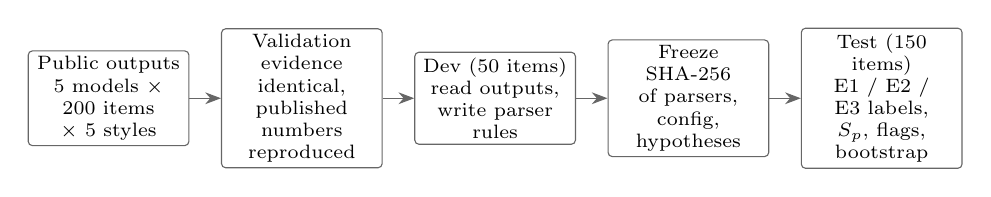
\begin{tikzpicture}[node distance=4mm, every node/.style={font=\scriptsize, align=center}, box/.style={draw=black!60, rounded corners=1.5pt, minimum height=8mm, inner sep=2pt, text width=19mm}]
\node[box] (a) {Public outputs\\5 models $\times$ 200 items\\$\times$ 5 styles};
\node[box, right=of a] (b) {Validation\\evidence identical,\\published numbers\\reproduced};
\node[box, right=of b] (c) {Dev (50 items)\\read outputs,\\write parser rules};
\node[box, right=of c] (d) {Freeze\\SHA-256 of parsers,\\config, hypotheses};
\node[box, right=of d] (e) {Test (150 items)\\E1 / E2 / E3 labels,\\$S_p$, flags, bootstrap};
\foreach \x/\y in {a/b,b/c,c/d,d/e} \draw[-{Stealth[length=2mm]}, black!60] (\x) -- (\y);
\end{tikzpicture}
\caption{Analysis pipeline. No model was called; every number derives from the recorded outputs.}\label{fig:pipeline}
\end{figure}

\subsection{Answer parsers}\label{sec:parsers}
Each output is mapped to yes, no, maybe or INVALID. \textbf{E1 strict} accepts only an output that is exactly one of the three words, ignoring case and surrounding punctuation; this is the rigid matching criticised by \cite{hua2025flaw}. \textbf{E2 substring} is the published extractor: ``yes'' anywhere, else ``no'' anywhere, else ``maybe'' anywhere. \textbf{E3 word-boundary} (ours, primary) takes the first whole-word yes/no/maybe and maps explicit hedges (``unclear'', ``insufficient'', ``not enough'', ``does not provide enough'', \ldots) to maybe when they come first. E2 and E3 differ in one way that matters: ``no'' is a substring of ``not'', ``cannot'' and ``know''.

\subsection{Metrics}\label{sec:metrics}
For one model and item, $C_1,\ldots,C_5$ are the five labels. Two distances instantiate Eq.~\ref{eq:sp}: $D_{cat}(a,b)=[a\neq b]$, and an ordinal $D_{ord}$ with yes--no $=1$, yes--maybe $=$ no--maybe $=0.5$ and INVALID at distance~1 from everything. $\bar C$ is the label that minimises the summed distance; under $D_{cat}$ it is the majority and $S_p$ is the majority share. INVALID counts as its own category in the primary analysis, so a non-answer can never agree with an answer. An item is \emph{fully stable} if all five labels are the same valid conclusion. It shows a \emph{polarity reversal} if it receives both yes and no. It shows an \emph{uncertainty shift} if it receives maybe and one definite answer without a reversal. It shows \emph{format instability} if INVALID occurs next to a valid label. Accuracy is the share of outputs that match gold, averaged over styles. We also report the published consistency definition and the label-free sensitivity and class-wise consistency of Errica et al.\ \cite{errica2025sensitivity}. Disagreement is the share of unordered pairs with different labels. \emph{Prompt-induced} disagreement is computed across the five styles within a model; \emph{model-induced} disagreement is computed across models within a style. Intervals are 95\% percentile bootstraps over test items (10,000 resamples, seed 2026), paired when two parsers are compared.

\paragraph{Prespecified expectations.} \textbf{H1}: every model changes conclusion on at least one test item. \textbf{H2}: for at least one model, switching from E3 to E2 moves $S_p$ or the reversal rate by at least 0.02. \textbf{H3}: accuracy and stability rank the instruction-following models differently.

%====================================================================
\section{Baseline Reproduction}\label{sec:baseline}
Before any new analysis we recomputed the source study's PubMedQA summary from raw outputs (Table~\ref{tab:repro}). We did this twice: from the stored extracted labels and from raw text with our re-implementation of E2. Both runs matched all \ReproCells{} published cells (consistency, its standard deviation, fully consistent count, accuracy, UNKNOWN rate and five per-style accuracies, for five models). The published consistency divides the majority count by all five styles but excludes UNKNOWN from the vote, so Meditron's near-total failure appears as consistency 0.01. The AI-generated agreement scripts from our planning prompts (Prompts 08, 09, 13) ran unchanged on our test labels, and their mean item agreement equals our $S_p(D_{cat})$ to machine precision (\texttt{results/logs/02}). Six unit tests, including the toy cases those prompts specified, pass (\texttt{results/logs/01}).

\begin{table}[t]
\caption{Reproduction of the published PubMedQA summary (all 200 items, E2 labels, published metric definitions). Every cell equals the published value.}\label{tab:repro}
\footnotesize\setlength{\tabcolsep}{4pt}
\begin{tabular}{@{}lrrrrrrrrr@{}}
\toprule
& Consist. & Full & Acc.\,\% & Unk.\,\% & orig. & formal & simpl. & role & direct \\
\midrule
\inputtab generated/tab_repro.tex
\bottomrule
\end{tabular}
\end{table}

%====================================================================
\section{Results}\label{sec:results}
\subsection{RQ1: conclusions change, mostly in stated uncertainty}\label{sec:rq1}
Table~\ref{tab:main} gives the primary results. H1 holds. With evidence and question fixed, each instruction-following model gave more than one conclusion on 46\% (Mistral) to 61\% (Phi-3 Mini) of test items. No model was fully stable on more than \FullMistral{} of items. Figure~\ref{fig:types} shows that the kind of change differs sharply by model. For Phi-3 Mini and Gemma~2 the dominant change is an uncertainty shift: one style yields ``maybe'' and another a definite answer. Llama~3.2 is the only model with frequent polarity reversals (\RevLlama{} of items, CI in the released tables). Gemma~2 and Mistral almost never reverse, but they also almost never answer ``no'' (\NoGemma{} and \NoMistral{} of their outputs). Mistral's largest instability is in format: \FmtMistral{} of items contain a non-answer next to an answer. Table~\ref{tab:examples} shows real outputs.

\begin{table}[t]
\caption{Conclusion stability on the \NTest{} test items (E3 parser). $S_p$ with 95\% bootstrap CI. ``Changed'' = more than one label across the five styles. Flags are shares of items. Valid = share of outputs with a yes/no/maybe conclusion.}\label{tab:main}
\footnotesize\setlength{\tabcolsep}{3.2pt}
\begin{tabular}{@{}lrrrrrrrrr@{}}
\toprule
Model & $S_p$ ($D_{cat}$) & \shortstack[r]{$S_p$\\($D_{ord}$)} & Changed & \shortstack[r]{Fully\\stable} & Reversal & \shortstack[r]{Unc.\\shift} & Format & Valid & Acc. \\
\midrule
\inputtab generated/tab_main.tex
\bottomrule
\end{tabular}
\end{table}

\begin{figure}[t]
\centering
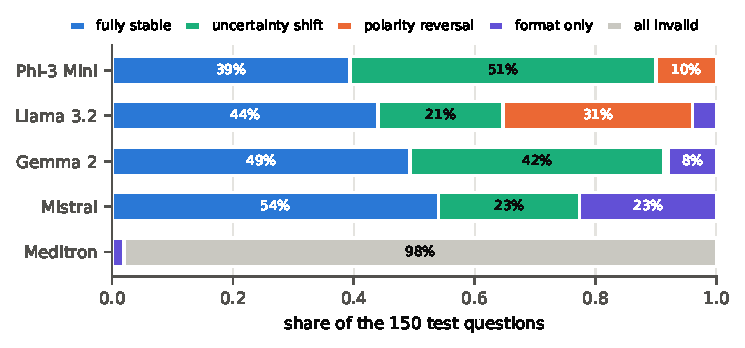
\includegraphics[width=0.78\linewidth]{figures/fig_item_types.pdf}
\caption{Outcome per test item, classes mutually exclusive in the order listed (a reversal item may also contain ``maybe''). Same evidence, same question, five prompt styles.}\label{fig:types}
\end{figure}

\begin{table}[t]
\caption{Real outputs (first 10 tokens, cut at 34 characters) for three test items with a polarity reversal. Label = E3 conclusion.}\label{tab:examples}
\small
\begin{tabular}{@{}llL{0.45\linewidth}l@{}}
\toprule
Model / item & Style & Output & Label \\
\midrule
\inputtab generated/tab_examples.tex
\bottomrule
\end{tabular}
\end{table}

Under $D_{ord}$, where a move to ``maybe'' costs half a reversal, Phi-3 Mini and Gemma~2 look clearly more stable (0.90--0.91) and Llama~3.2 stays lowest (\SpOrdLlama). The review's distinction is therefore visible in the data: an uncertainty shift and a reversal are different inferential failures, and a 0/1 distance hides which one occurred.

\subsection{RQ2: the parser changes what is measured}\label{sec:rq2}
Table~\ref{tab:evaluators} and Figure~\ref{fig:evaluators} score the same \NOutTest{} test outputs with the three parsers. \textbf{E1 strict} treats \EoneInvalidFunc{} of instruction-following outputs as INVALID, because models write ``Yes.\ The study\ldots'' instead of a bare word. This lowers $S_p$ by between 0.05 (Phi-3 Mini) and 0.31 (Gemma~2) and accuracy by up to 31 points (Phi-3 Mini: \AccEonePhi{} vs.\ \AccPhi). It also changes the ranking. Under E1, Phi-3 Mini is the \emph{most} stable instruction-following model and its reversals disappear (0\% vs.\ \RevPhi), because most of its definite answers become invalid. Under rigid matching, ``prompt sensitivity'' is largely sensitivity in output \emph{format}, which is what Hua et al.\ \cite{hua2025flaw} argued.

\textbf{E2 substring} disagrees with E3 on only \EtwoEthreeDis{} test outputs, yet the disagreement is systematic. In \EtwoMaybeNo{} cases an answer that begins ``Maybe'' and goes on to say the context ``does not'' state something is read as ``no''. In \EtwoInvalidNo{} cases a non-answer such as ``The excerpt doesn't provide enough information\ldots'' is read as ``no''. Overall $S_p$ moves by at most 0.013, so E2 looks harmless if only $S_p$ is reported. The \emph{type} of instability changes, however. Mistral's uncertainty-shift rate rises from \UncMistral{} to \UncEtwoMistral{} ($+$10.0 points, paired CI [\dUncEtwoLoMistral, \dUncEtwoHiMistral]). Phi-3 Mini's reversal rate rises from \RevPhi{} to \RevEtwoPhi{}. Accuracy is inflated by \dAccEtwoMistral{} points for Mistral (CI [\dAccEtwoLoMistral, \dAccEtwoHiMistral]), because 49 of the 150 test items have gold ``no'' and the parser converts hedges into ``no''. H2 is met at its threshold by one model only (Phi-3 Mini, 3 items, $\Delta=0.020$). We report it as weak support. The more important finding is the shift in instability type, which H2 did not anticipate.

\begin{table}[t]
\caption{The same test outputs under three parsers. Pub.\ = published consistency definition. Sens./Cons.\ = Errica et al.'s label-free sensitivity (normalised entropy, lower is better) and class-wise consistency \cite{errica2025sensitivity}.}\label{tab:evaluators}
\footnotesize\setlength{\tabcolsep}{3.5pt}
\begin{tabular}{@{}llrrrrrrrr@{}}
\toprule
Model & Parser & Valid & $S_p$ & Pub. & Reversal & \shortstack[r]{Unc.\\shift} & Acc. & Sens. & Cons. \\
\midrule
\inputtab generated/tab_evaluators.tex
\bottomrule
\end{tabular}
\end{table}

\begin{figure}[t]
\centering
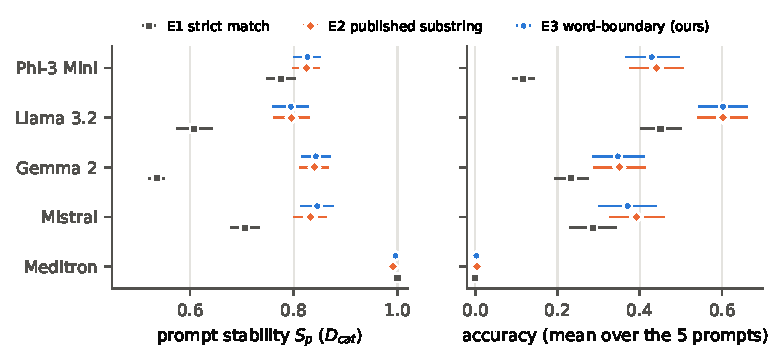
\includegraphics[width=0.85\linewidth]{figures/fig_evaluators.pdf}
\caption{Stability and accuracy of the same outputs under three parsers (95\% bootstrap CIs over test items).}\label{fig:evaluators}
\end{figure}

\paragraph{The distance definition is also an artifact.} Meditron answers almost nothing (\ValidMeditron{} valid). With INVALID as a category, its $S_p$ is \SpMeditron, the highest of all models, because it fails identically under every prompt. The published definition gives \PubMeditron. The label-free sensitivity of Errica et al.\ also calls Meditron the least sensitive model under every parser. A stability score that is reported without the valid-answer rate can therefore rank a non-functional model first.

\subsection{RQ3: stability, accuracy and what causes disagreement}\label{sec:rq3}
\paragraph{Accuracy versus stability.} H3 holds. Among the four instruction-following models, accuracy ranks Llama~3.2 $>$ Phi-3 Mini $>$ Mistral $>$ Gemma~2, while $S_p$ ranks them exactly in reverse (Kendall $\tau=\HthreeTau$; Figure~\ref{fig:accstab}). The bootstrap intervals of the three most stable models overlap, so the reversal is not itself a precise estimate. Table~\ref{tab:matrix} fills the review's accuracy--stability matrix (review Table~4). ``Stable but wrong'' is common: \SWGemma{} of 150 items for Gemma~2 and \SWMistral{} for Mistral, more than their stable-and-correct items. The label distributions explain why. Gemma~2 and Mistral answered ``maybe'' in \MaybeGemma{} and \MaybeMistral{} of outputs, although only 10 of 150 test items have gold ``maybe''. Of Gemma's stable-wrong items, \SWGemmaNoMaybe{} are gold-``no'' items answered ``maybe'' under all five prompts. Their high stability is largely stable abstention. Llama~3.2's stable errors lean the other way: all 14 are a stable ``yes'', including \SWLlamaNoYes{} gold-``no'' items. This matches the review's warning that consistency is not correctness (review \S5, Table~4). It also confirms the source study's conclusion that consistency and accuracy dissociate \cite{hariprasad2026clinical}, now on held-out items with a different parser.

\begin{figure}[t]
\centering
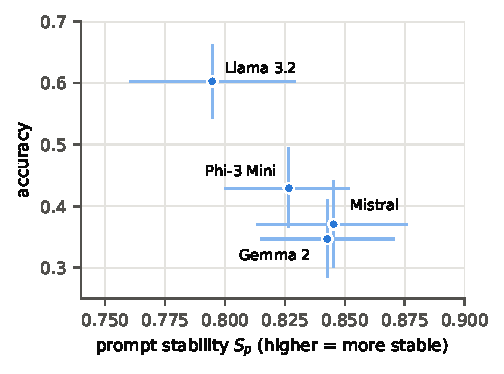
\includegraphics[width=0.45\linewidth]{figures/fig_acc_vs_stability.pdf}
\caption{Accuracy against conclusion stability, instruction-following models, test items (95\% CIs).}\label{fig:accstab}
\end{figure}

\begin{table}[t]
\caption{Accuracy--stability matrix (review Table~4) on 150 test items (stable = all five styles give the same valid conclusion; correct = majority conclusion matches gold), and each model's output label distribution.}\label{tab:matrix}
\footnotesize
\begin{tabular}{@{}lrrrrrrr@{}}
\toprule
& \multicolumn{4}{c}{Items (of 150)} & \multicolumn{3}{c}{Output labels} \\
\cmidrule(lr){2-5}\cmidrule(l){6-8}
Model & \shortstack[r]{Stable\\correct} & \shortstack[r]{Stable\\wrong} & \shortstack[r]{Unstable\\correct} & \shortstack[r]{Unstable\\wrong} & yes & no & maybe \\
\midrule
\inputtab generated/tab_matrix.tex
\bottomrule
\end{tabular}
\end{table}

\paragraph{Which prompts move the conclusion?} Figure~\ref{fig:variants} shows how often each style disagrees with the other four when those four agree. No style is uniformly worst. ``Direct'' is the most deviant for Phi-3 Mini (\DevPhiDirect) and Mistral (\DevMistralDirect), ``formal'' for Llama~3.2 (\DevLlamaFormal) and ``simplified'' for Gemma~2 (\DevGemmaSimplified). Roleplay is the least deviant style for Phi-3 Mini (\DevPhiRoleplay). The source study advised avoiding roleplay prompts \cite{hariprasad2026clinical}; our item-level view does not single it out. Part of the effect is format rather than meaning. Roleplay and direct are the two styles without an ``only yes/no/maybe'' line, and they are where Mistral's valid-answer rate falls to \ValidVarMistralDirect{}. For a single fixed prompt, accuracy varied by up to \AccRangePhi{} points across styles (Phi-3 Mini: \AccMinPhi{}--\AccMaxPhi). A one-prompt evaluation of these models could thus differ by more than 20 accuracy points depending only on the template.

\begin{figure}[t]
\centering
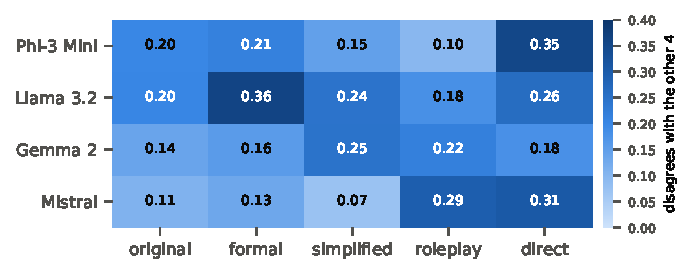
\includegraphics[width=0.6\linewidth]{figures/fig_variant_deviation.pdf}
\caption{Share of test items on which a style's conclusion differs from the (unique) majority of the other four styles.}\label{fig:variants}
\end{figure}

\paragraph{Prompt-induced versus model-induced disagreement.} The review's Eq.~6 separates variance from prompts and from models. Among the four instruction-following models, two prompts given to the same model disagreed on \PromptInd{} of pairs. Two models given the same prompt disagreed on \ModelInd{} of pairs (difference \PMdiff, CI [\PMlo, \PMhi]). Model choice moved conclusions more than wording did. Wording effects were still large: about one prompt pair in four disagreed although evidence and question were identical.

\paragraph{CSI weight sensitivity (G5).} We cannot compute the review's CSI. Outputs of 10 tokens carry no evidence citations, and we have no semantic judge. We can test its central assumption, that a weighted sum yields a stable ranking. Table~\ref{tab:csi} reports three measurable components: inferential agreement ($S_p$), uncertainty agreement (one minus the uncertainty-shift rate) and factual accuracy. Over 10,000 random weight vectors (Dirichlet(1,1,1)), \CSIorders{} distinct rankings of the four models occurred. Llama~3.2 ranked first under \CSItopLlama{} of weightings and Mistral under \CSItopMistral. Yet Llama~3.2 ranks \emph{last} on inferential agreement alone. Which model is ``most conclusion-stable'' is therefore a weighting decision, and the review's CSI needs its weights justified, or its components reported separately, before it can rank systems.

\begin{table}[t]
\caption{CSI-style components (test items, E3) and the share of 10,000 random weightings under which each model ranks first.}\label{tab:csi}
\small
\begin{tabular}{@{}lrrrr@{}}
\toprule
Model & $A_{inf}=S_p$ & $A_{unc}$ & $A_{fact}$ & Ranked first \\
\midrule
\inputtab generated/tab_csi.tex
\bottomrule
\end{tabular}
\end{table}

\subsection{Robustness}\label{sec:robust}
Roleplay adds a persona and drops the ``only'' format line, so it is arguably not meaning-preserving (review \S8.5). Without it (Table~\ref{tab:robust}), Mistral's $S_p$ rises from \SpMistral{} to \SpNoRoleMistral{} and Llama~3.2's reversal rate falls from \RevLlama{} to \RevNoRoleLlama{}. Phi-3 Mini's $S_p$ falls slightly, and all qualitative findings remain. Dropping the item with the false-positive leakage hit changes no value by more than 0.005 (\texttt{results/tables/robustness.csv}). The E2 and E1 columns repeat RQ2: E2 barely moves $S_p$, while E1 changes both its level and the model order.

\begin{table}[t]
\caption{Robustness of $S_p$ ($D_{cat}$) and the reversal rate (test items).}\label{tab:robust}
\small
\begin{tabular}{@{}lrrrrrr@{}}
\toprule
& \multicolumn{4}{c}{$S_p$} & \multicolumn{2}{c}{Reversal} \\
\cmidrule(lr){2-5}\cmidrule(l){6-7}
Model & E3, 5 styles & E3, no roleplay & E2 & E1 & 5 styles & no roleplay \\
\midrule
\inputtab generated/tab_robust.tex
\bottomrule
\end{tabular}
\end{table}

\subsection{Hypotheses}
\textbf{H1 supported}: every model changed conclusion on some items (Meditron on 2\%, the others on 46--61\%). \textbf{H2 supported only at its threshold}: one model and three items. The reversal-rate difference is exactly $3/150=0.02$. Our script first reported it as unmet because of a floating-point comparison; the fix is logged in \texttt{results/logs/09}. \textbf{H3 supported}: the rankings are reversed. The intervals around the stability ranking overlap, however.

%====================================================================
\section{Discussion}\label{sec:discussion}
\paragraph{What the review got right.} Holding evidence fixed and changing only instruction and format changed the stated conclusion on about half of the items for every working model. This is the inferential instability the review set out to define. Accuracy and stability came apart, as the review's Table~4 anticipated, and the parser changed the measurement, as \S7.3 warned.

\paragraph{What the review should revise.} First, a single $S_p$ hides the distinction that matters most for research conclusions. A shift from ``supports'' to ``insufficient evidence'' is a calibration problem. A shift from ``supports'' to ``contradicts'' is a reversal. The two occur in very different proportions across models, so a stability report should give both. Second, Eq.~7 needs a fixed $D$, a fixed $\bar C$ and an explicit rule for non-answers. Without them the same outputs give Meditron 0.996 or 0.004. Third, the CSI cannot be used to rank systems until its weights are justified; here the leader depended on the weights. Fourth, stability is not a virtue on its own. The most stable working models were stable because they abstained, and abstention was wrong on most items where the gold conclusion was definite.

\paragraph{Practical recommendation.} A study that uses an LLM to state conclusions from evidence should (i) run several meaning-preserving prompts and report the spread of conclusions, not one; (ii) report reversal and uncertainty-shift rates separately; (iii) report the valid-answer rate and the parser, and check the parser on held-out outputs; (iv) report accuracy against an independent label next to stability.

%====================================================================
\section{Threats to Validity}\label{sec:threats}
\textbf{Sampling variance (G3).} The source ran each prompt once at temperature~0. The data therefore cannot separate prompt effects from decoding or run-to-run noise; temperature-0 inference in Ollama is not guaranteed to be bit-identical. Sampling-based aggregation such as self-consistency \cite{wang2023selfconsistency} could not be studied either. The review's $V_{sampling}$ remains untested, and repeated runs are the first follow-up. \textbf{Output truncation.} Outputs were capped at 10 tokens, so some answers end before the conclusion (``Based on the provided excerpt, the study''). These count as INVALID, which inflates format instability, especially for Mistral. \textbf{Evidence quality.} The evidence is cut at 1,000 characters for most items and includes a dictionary wrapper, so the abstract's results are sometimes missing. This affects accuracy but not the within-item comparison, because every style saw the same text. \textbf{Prompt equivalence.} Styles differ in persona and format line, so not every difference is pure rewording. The no-roleplay analysis addresses this only partly. \textbf{Parser validity.} E3 was written by us. Its rules were fixed on development items, but no human labels exist yet. We provide a seeded sample of \AnnN{} test outputs, 40 of them E2/E3 disagreements, with a sealed key for blind annotation (\texttt{annotation/}). \textbf{Scope.} The data cover small models, one biomedical task, three-way conclusions and 150 test items. Larger models and free-text conclusions may behave differently. Only 10 test items have gold ``maybe'', so per-class results for ``maybe'' are imprecise. \textbf{Licence.} The source repository has no licence file. We redistribute none of its outputs; a script fetches them at the pinned commit.

%====================================================================
\section{Conclusion}\label{sec:conclusion}
On public outputs with fixed evidence, meaning-preserving prompt changes altered the conclusion of every working model on about half of the items. Mostly the change was in stated uncertainty; for one model it often reversed polarity. How large this instability looks depended on the parser and on the treatment of non-answers. Stability ranked the models in the opposite order to accuracy, and a CSI-style composite ranked them differently under different weights. The review's framework is measurable, but the stability number is only one part of the report. It needs the parser, the distance definition, the separate reversal and uncertainty-shift rates, the valid-answer rate and accuracy. Three follow-ups remain open: repeated runs to estimate sampling variance, human labels to validate the parser, and longer outputs from larger models with cited evidence so that the evidence and semantic components of the CSI can be measured.

\begin{acks}
Outputs, prompts and the PubMedQA sample are from the public repository of S.~Hariprasad. AI assistance (planning prompts, code drafting, editing) is disclosed in \texttt{ai\_assistance\_log.md}; every number in this paper is generated by the released scripts from the recorded outputs.
\end{acks}

\bibliographystyle{ACM-Reference-Format}
\bibliography{references}

\appendix
\section{Reproducibility}
\texttt{bash scripts/fetch\_data.sh} clones the source repository at commit \texttt{4c82a7b6} into \texttt{data\_raw/}. \texttt{bash scripts/run\_all.sh} then runs tests, validation, reproduction, the starter-code check, the analysis, the figures and the tables, and writes all logs to \texttt{results/logs/}. The run takes under one minute on a laptop CPU and needs Python with pandas, NumPy, SciPy and Matplotlib. No API keys or GPU are needed. A run from a fresh copy reproduced every table byte for byte (\texttt{results/logs/12\_fresh\_copy\_reproduction.log}).
\end{document}
